\chapter {GIỚI THIỆU}

Bạn có biết rằng, bạn vẫn đang sử dụng phương pháp Cây quyết định (Decision Tree) để đưa ra quyết định trong cả cuộc đời mà không hề hay biết. Hãy xem xét tình huống một người yêu cầu bạn cho họ mượn xe trong một ngày và bạn phải đưa ra quyết định có cho họ mượn xe hay không. Có một số yếu tố giúp xác định quyết định của bạn, một số yếu tố đã được liệt kê bên dưới:

\begin{enumerate}
    \item Người này là bạn thân hay chỉ là người quen? Nếu người đó chỉ là người quen, hãy từ chối yêu cầu; nếu người đó là bạn thì hãy chuyển sang bước tiếp theo.
    \item Người này hỏi mượn xe lần đầu? Nếu vậy, hãy cho họ mượn xe, nếu không thì chuyển sang bước tiếp theo.
    \item Lần trước họ trả xe có bị hư không? Nếu có, hãy từ chối yêu cầu; nếu không, hãy cho họ mượn xe.
\end{enumerate}

Decision Tree cho tình huống nói trên trông giống như sau:

\begin{center}
    \begin{figure}[h!]
        \begin{center}
         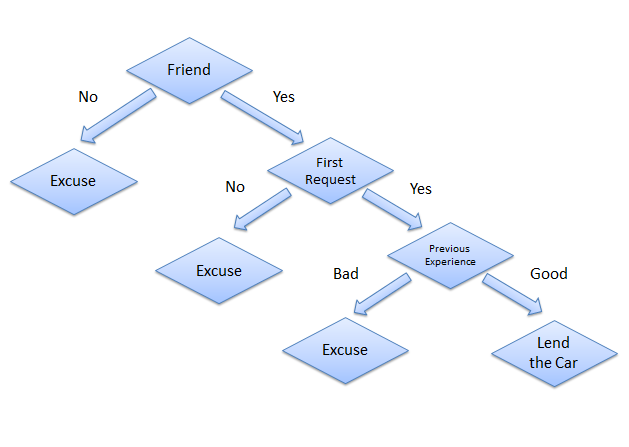
\includegraphics[scale=0.7]{chapter1/img/dt_ex1.png}
        \end{center}
        \caption{Ví dụ về việc ra quyết định dựa trên các câu hỏi.}
        \label{fig:dt_ex1}
    \end{figure}
\end{center}
